\documentclass[shortpres]{beamer}
\usetheme{CambridgeUS}

% Depending on build configuration, one of these packages will
% enable unicode
%\usepackage[utf8]{inputenc}
\usepackage{fontspec}


%Images
\usepackage{graphicx, svg}

%Showing movies and gifs
%\usepackage{animate, media9, movie15}
\usepackage{animate}
\usepackage{array}

\usepackage{caption}
%\usepackage{subcaption}
\usepackage{multicol}
\usepackage{color}
\usepackage{pgfplots}
\usepackage{xmpmulti}

\usepackage{algorithm,algpseudocode}  %for algorithm environment

\setbeamertemplate{footline}
{
	\leavevmode%
	\hbox{%
		\begin{beamercolorbox}[wd=.333333\paperwidth,ht=2.25ex,dp=1ex,center]{author in head/foot}%
			\usebeamerfont{author in head/foot}\insertshortauthor%~~\beamer@ifempty{\insertshortinstitute}{}{(\insertshortinstitute)}
		\end{beamercolorbox}%
		\begin{beamercolorbox}[wd=.333333\paperwidth,ht=2.25ex,dp=1ex,center]{title in head/foot}%
			\usebeamerfont{title in head/foot}\insertshorttitle
		\end{beamercolorbox}%
		\begin{beamercolorbox}[wd=.333333\paperwidth,ht=2.25ex,dp=1ex,right]{date in head/foot}%
			\usebeamerfont{date in head/foot}\insertshortdate{}\hspace*{2em}
			\insertframenumber{} / \inserttotalframenumber\hspace*{2ex}
	\end{beamercolorbox}}%
	\vskip0pt%
}\part{title}
\beamertemplatenavigationsymbolsempty


%color specification---------------------------------------------------------------
\definecolor{TUMblue}{rgb}{0.00, 0.40, 0.74}
\definecolor{TUMgray}{rgb}{0.85, 0.85, 0.86}
\definecolor{TUMpantone285C}{rgb}{0.00, 0.45, 0.81}
\definecolor{lightblue}{rgb}{0.7529,0.8118,0.9333}

\setbeamercolor{block title}{fg=white, bg=TUMpantone285C}
\setbeamercolor{block body}{bg=lightblue}
\setbeamertemplate{blocks}[rounded][shadow=true]
%----------------------------------------------------------------------------------

\setbeamercolor{frametitle}{fg=TUMblue, bg=white}
\setbeamercolor{palette primary}{fg=TUMblue,bg=TUMgray}
\setbeamercolor{palette secondary}{use=palette primary,fg=TUMblue,bg=white}
\setbeamercolor{palette tertiary}{use=palette primary,fg=white, bg=TUMblue}
\setbeamercolor{palette quaternary}{use=palette primary,fg=white,bg=TUMpantone285C}


\setbeamercolor{title}{bg=white,fg=TUMblue}
\setbeamercolor{item projected}{use=item,fg=black,bg = lightblue}
\setbeamercolor{block title}{fg=black, bg=lightblue}
\setbeamercolor{block body}{bg=white}
\setbeamertemplate{blocks}[rounded][shadow=true]
%----------------------------------------------------------------------------------



%############### Self defined commands ##############################
\newcommand{\imgvoffset}{-20pt}
\newcommand{\texthoffset}{20pt}
\newcommand{\imgfullscale}{0.75}
%####################################################################

\usepackage{anyfontsize}

\title[{Tsunami simulation}]{Assignment 1}

<<<<<<< HEAD
\author[Bellamy Honal, Wieser]{George Bellamy, Christoph Honal, Felix Wieser\newline\vspace{10pt}{\small Bachelorpraktikum}}
=======
\author[Bellamy Honal, Wieser]{George Bellamy, Christoph Honal, Felix Wieser\\\vspace{10pt}{\small Bachelorpraktikum}}
>>>>>>> b2b50e45a52d959e13c6bd0555215228f0821f0f
\institute[TU M\"unchen]{Techncal University of Munich}

\date{7. November 2017}

\begin{document}
\maketitle

\begin{frame}{Solver implementation: Core functionality}
	\begin{multicols}{2}
		\begin{figure}[t]
			%\includesvg{img/FCalc}
			\caption*{FCore}			
		\end{figure}

		\columnbreak
		
		\begin{figure}[t]
%			\includesvg{img/FCalc}
			\caption*{FCalc}
		\end{figure}

	\end{multicols}
	\begin{tabular}{ll}
		FWave & Solver of the 2D-Problem\\
		FCore & Implementation of NetUpdates and eigenvalues computation\\
		FCalc & Supplemental methods (average height, ...)\\
		FCoreTests & Testing of all implemented functionality
	\end{tabular}
\end{frame}

\begin{frame}{Solver implementation: Testing}
	\begin{multicols}{2}
		
		\begin{figure}
%			\includesvg{}
			\caption*{FCoreTests}
		\end{figure}
		
		\columnbreak
		
		Tests cover
		\begin{itemize}
			\item Core functionality
			\item Eigenvalue computation
			\item Supplemental methods in FCalc
			\item Comparison with precomputed data
		\end{itemize}
	\end{multicols}
\end{frame}

\begin{frame}{Shock-Shock Problem}
	\begin{figure}[t]
		\vspace{\imgvoffset}
		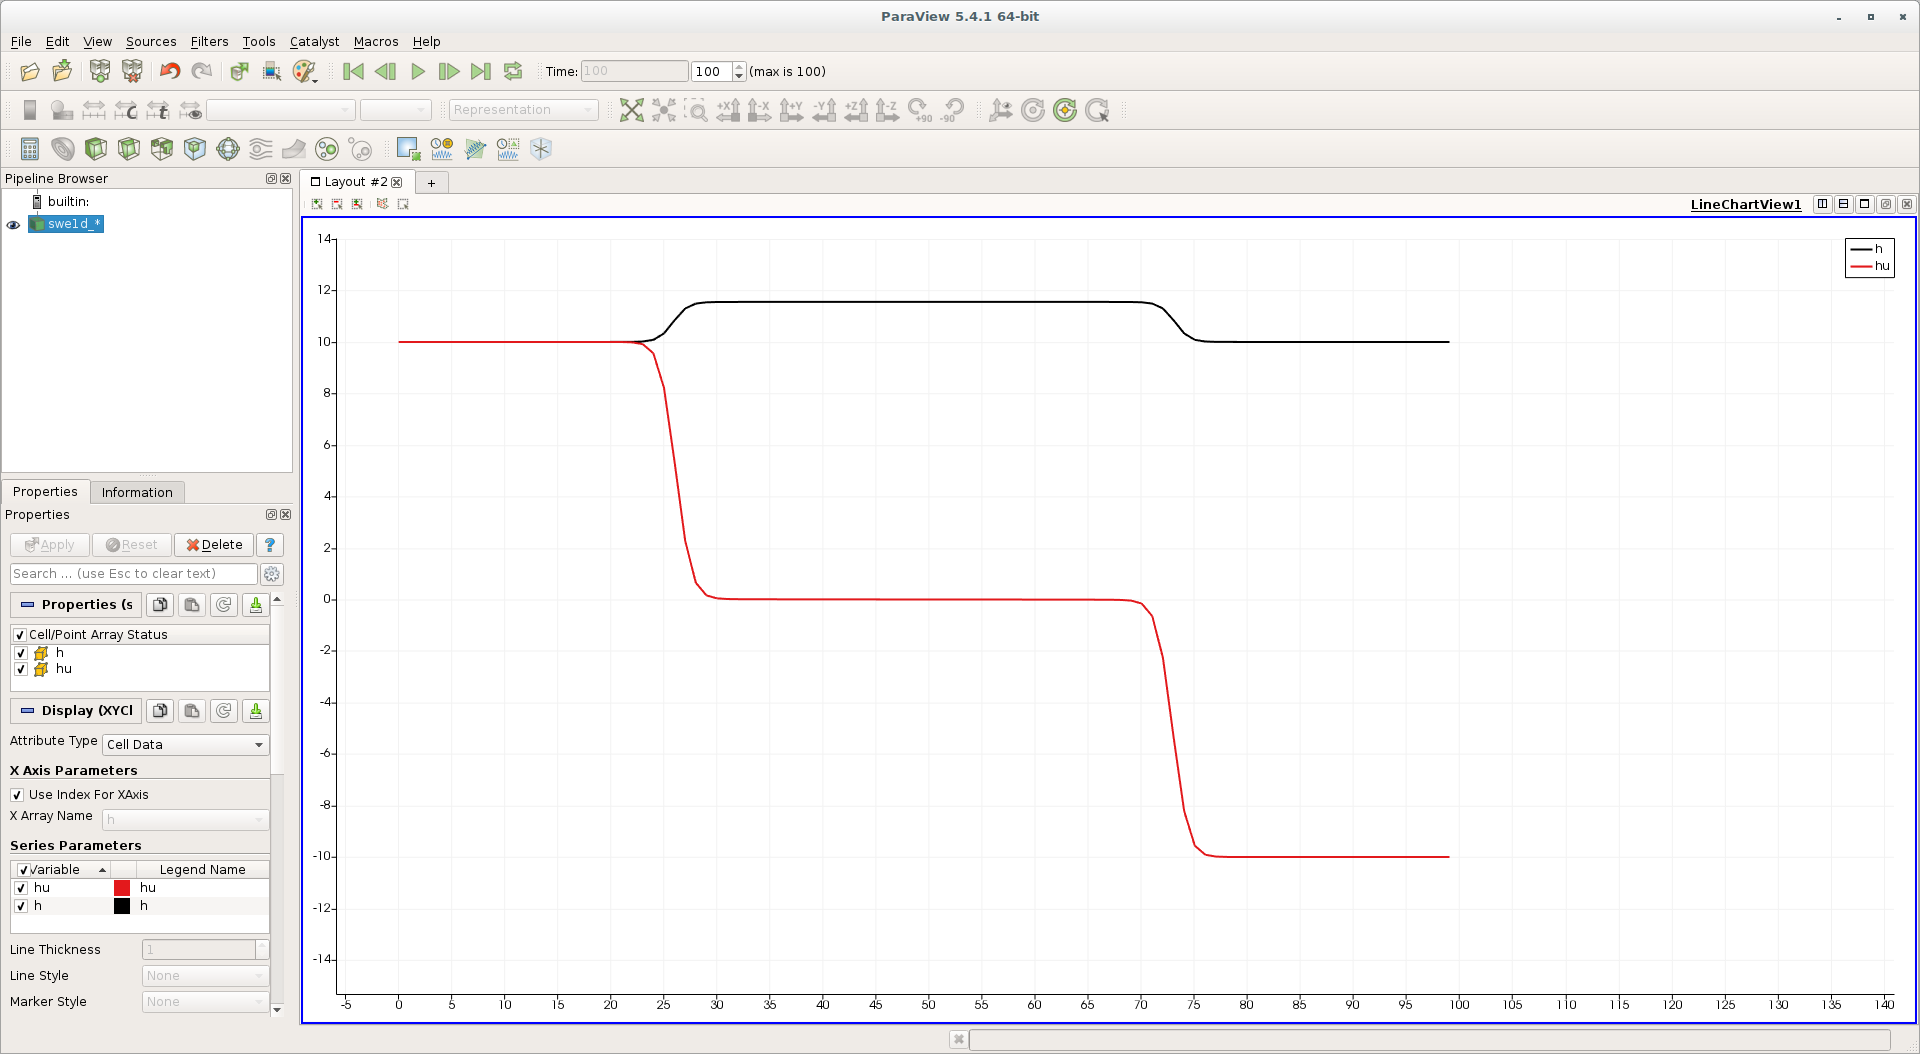
\includegraphics[clip, width=\imgfullscale\linewidth]{img/Shock-Shock.png}
		\caption*{Shock-Shock problem}
	\end{figure}
	%TODO: Add text
	Some random text
\end{frame}

\begin{frame}{Rare-Rare Problem}
	\begin{figure}[t]
		\vspace{\imgvoffset}
		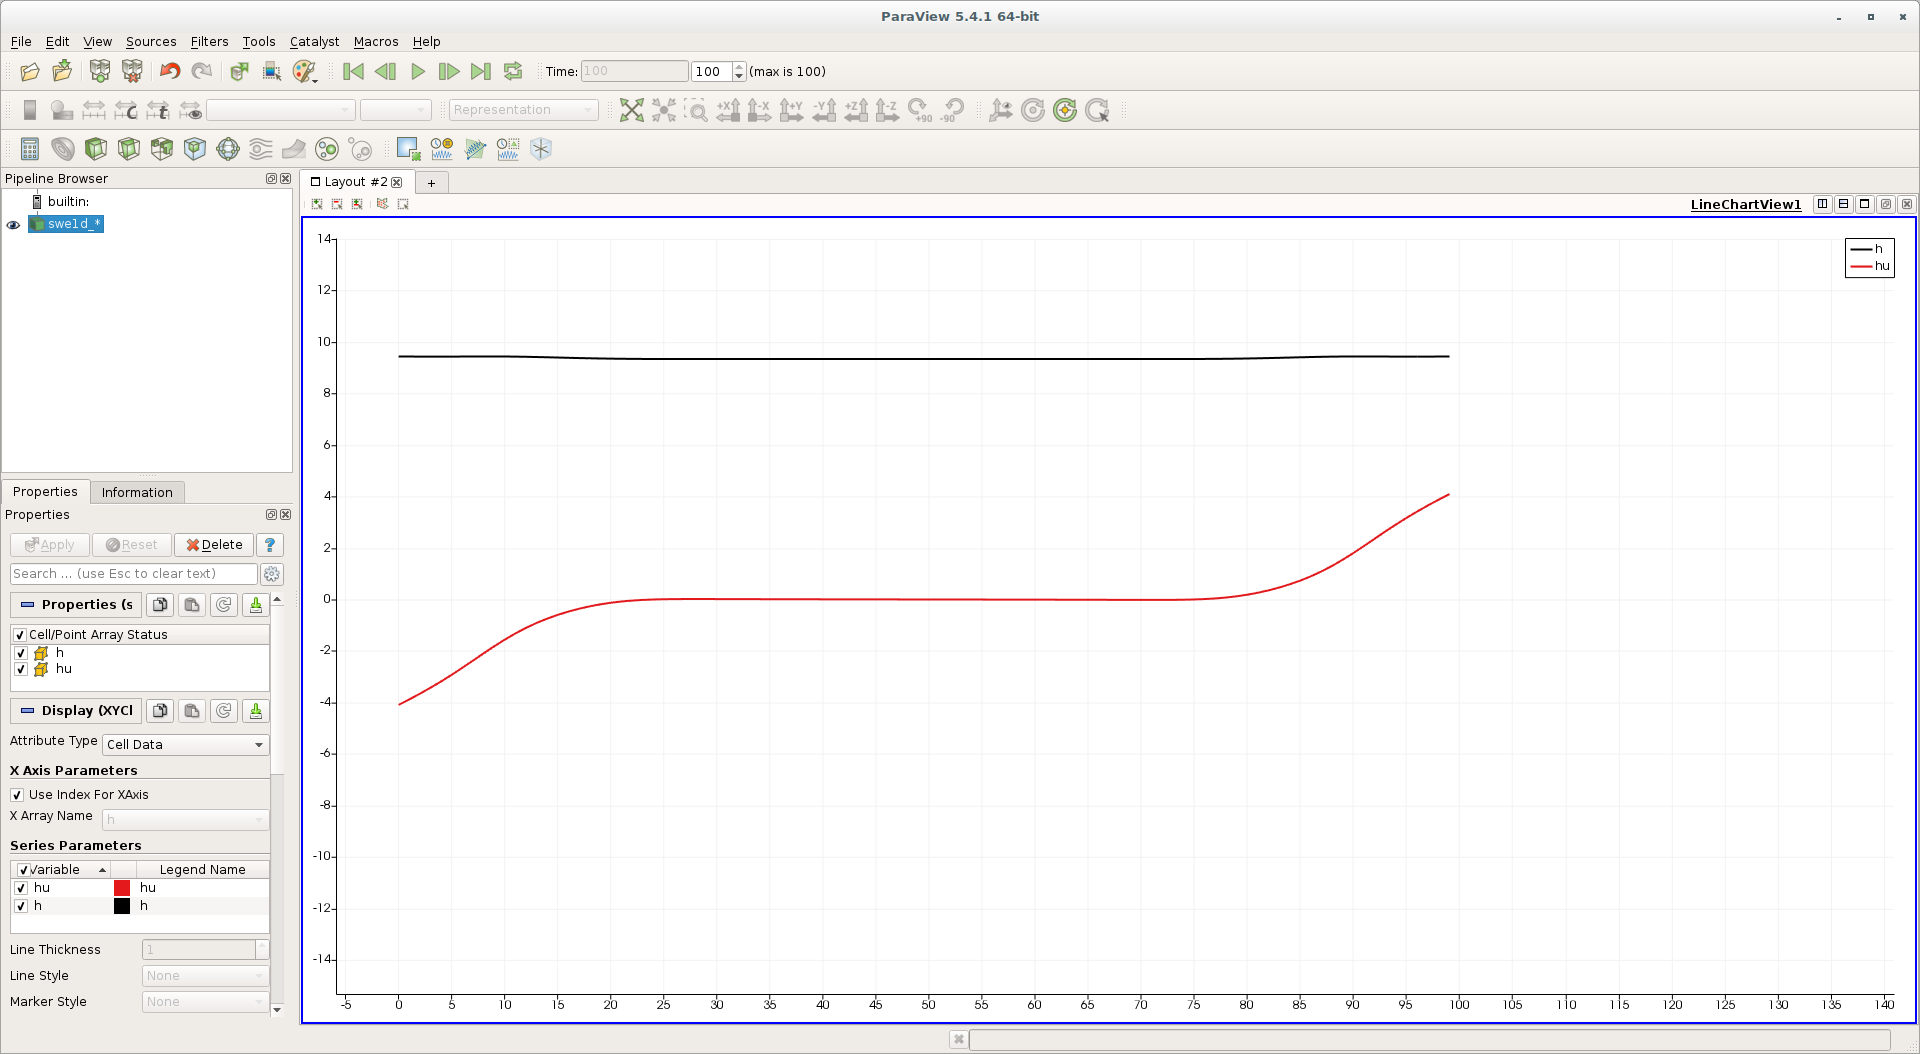
\includegraphics[clip, width=\imgfullscale\linewidth]{img/Rare-Rare.png}
		\caption*{Rare-Rare problem}
	\end{figure}
	%TODO: Add text
	Some random text
\end{frame}

\begin{frame}{Dam-Break: When does the water arrive?}
	\begin{figure}[t]
		\vspace{\imgvoffset}
		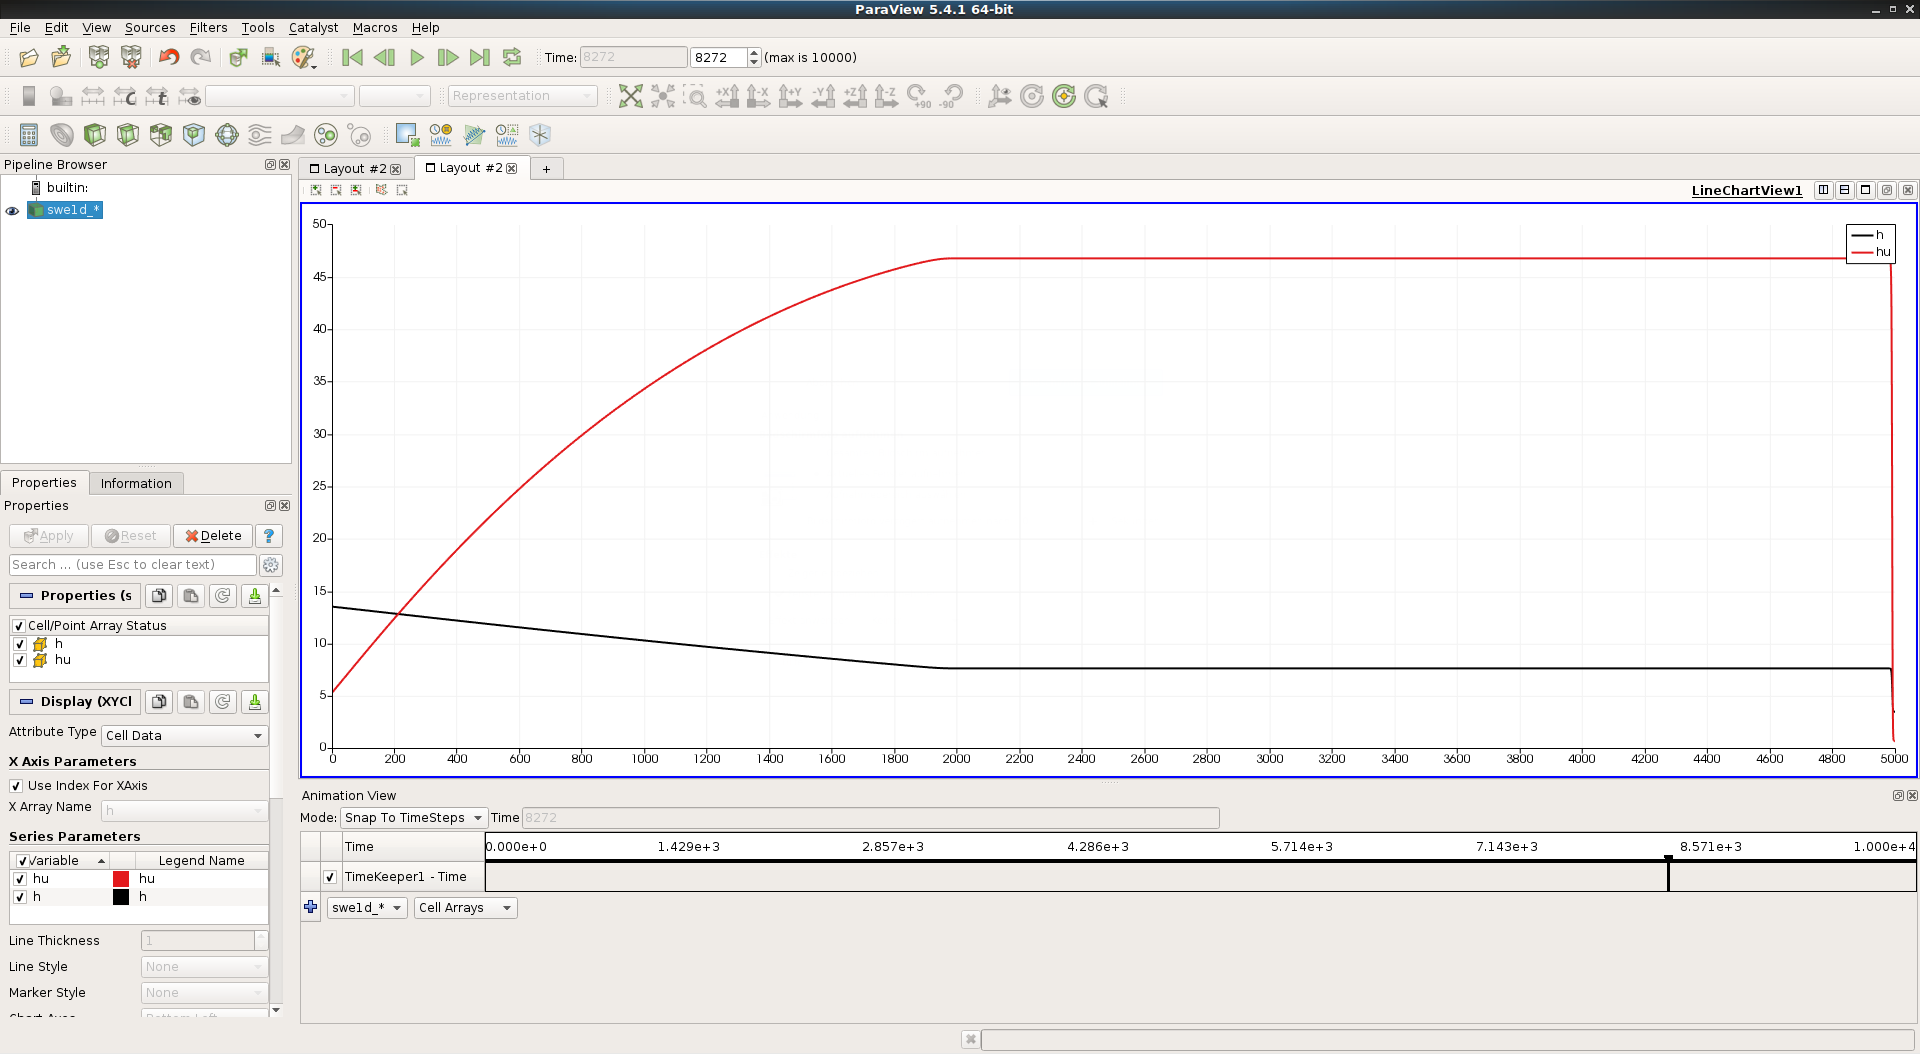
\includegraphics[width=\imgfullscale\linewidth]{img/4_dorf_arrival_as_graph.png}
		\caption*{Arrival of the wave at the village}
	\end{figure}
	The wave arrives after $\approx$ $7,3$ minutes at the village
\end{frame}

\begin{frame}{Dam-Break: Scenario 1}
	\begin{figure}[t]
		\vspace{\imgvoffset}
		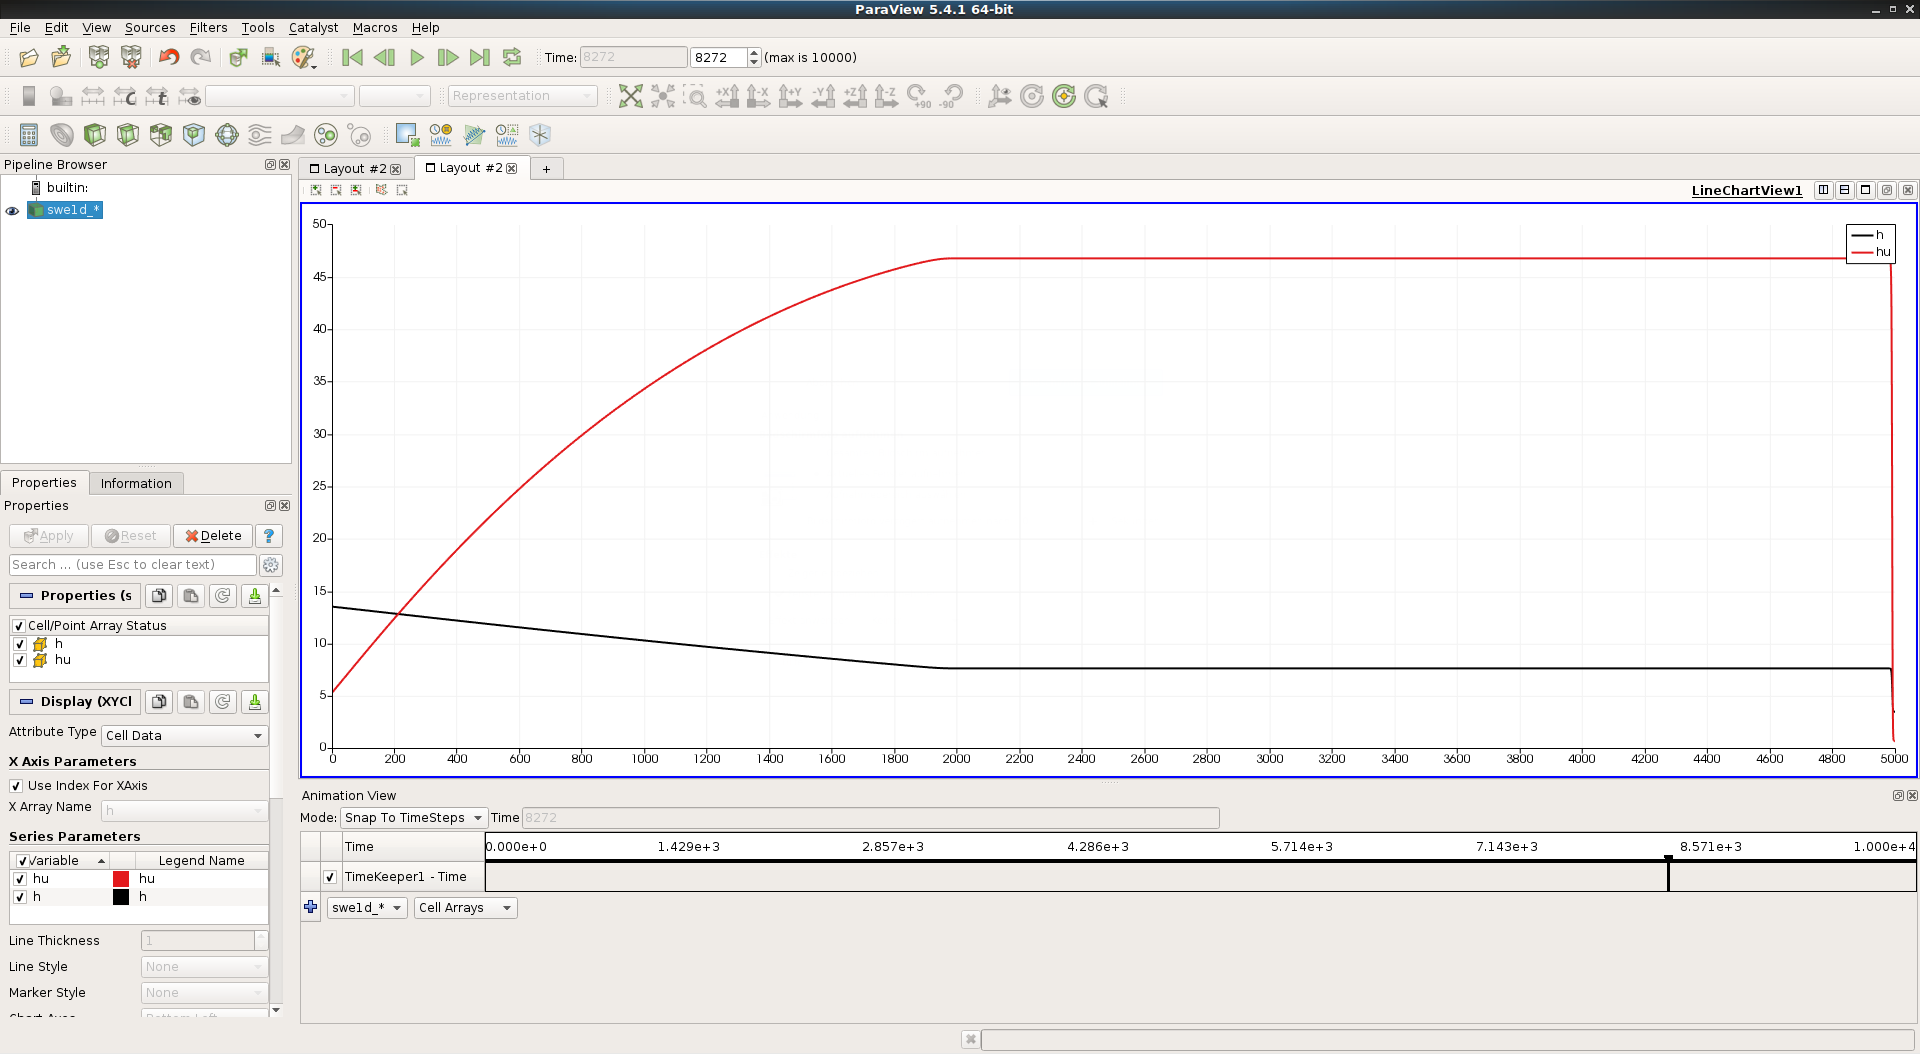
\includegraphics[width=\imgfullscale\linewidth]{img/4_dorf_arrival_as_graph.png}
		\caption*{Scenario visualisation}
	\end{figure}
	
	\begin{tabular}{m{3cm} m{\linewidth-5cm}}
		$
		\begin{matrix}
		h_l & = & 42\\
		h_r & = & 42
		\end{matrix}
		$
		&
		%TODO Add description here
		Add description here
	\end{tabular}
\end{frame}

%TODO: Add slide for each scenario...

%TODO: Remove / comment the following slides, when finished
\begin{frame}{Template: image centered, text below}
	\begin{figure}[t]
		\vspace{\imgvoffset}
		
\includegraphics[clip, width=\imgfullscale\linewidth]{img/dummy_image.jpg}
		\caption*{Dummy image}
		Die Crash Test Dummies sind eine um 1840 gegründete, weltweit operierende Gang von Verkehrssündern. Zahlreiche, teils spektakuläre, Unfälle gehen auf das Konto dieser von Interpol, CIA und FDP gesuchten Organisation (stupidedia.org)
	\end{figure}
\end{frame}

\begin{frame}{Template: content left, content right}
	\begin{multicols}{2}
		\begin{figure}[t]
			
\includegraphics[clip, width=0.98\linewidth]{img/dummy_image.jpg}
			\caption*{Dummy image}
		\end{figure}		
		
	\columnbreak
	
		Die Crash Test Dummies sind eine um 1840 gegründete, weltweit operierende Gang von Verkehrssündern. Zahlreiche, teils spektakuläre, Unfälle gehen auf das Konto dieser von Interpol, CIA und FDP gesuchten Organisation (stupidedia.org)
	\end{multicols}
\end{frame}

\begin{frame}{Mathegedöns}
	\begin{multicols}{2}
		
		Aufzählung
		\begin{itemize}
			\item Das ist
			\item eine wirklich
			\item sinnvolle Aufzählung
		\end{itemize}
		
		\vspace{10pt}
		
		Nummerierung
		\begin{enumerate}
			\item Eins
			\item Zwei
			\item Drölf
		\end{enumerate}
		
		\vspace{10pt}
		
		\begin{tabular}{ll}
			Name & Leistung\\
			\hline
			Heinz & Nicht so toll\\
			Anton & Besser\\
			Julian & Alles gewonnen (Streber)
		\end{tabular}
		
	\columnbreak
		
		Matrix \hspace{10pt}
		$
			\begin{bmatrix}
				a & b & c\\
				d & e & f\\
				g & \dots & 42
			\end{bmatrix}
			\cdot
			\begin{pmatrix}
			a & b & c\\
			d & e & f\\
			g & \dots & 42
			\end{pmatrix}
			\cdots
		$
		
	\end{multicols}
	
\end{frame}
\end{document}